\documentclass[a4paper]{article}
\title{Simulating calcium buffering and handling at nerve terminals with CellBlender/MCell}
\author{Jaron Lee}
\usepackage{mathtools}
\usepackage{graphicx}
\usepackage{siunitx}
\usepackage{natbib}
\usepackage{hyperref}
\usepackage{tabularx}
\usepackage{enumerate}
\usepackage{extarrows}
\usepackage[hmargin=3cm,vmargin=3.5cm]{geometry}
\usepackage{amssymb}
\usepackage{amsmath}
\usepackage{float}
\setlength\parindent{0pt} % sets indent to zero
\setlength{\parskip}{10pt} % changes vertical space between paragraphs
\renewcommand\thesubsection{\thesection.\roman{subsection}}
\makeatletter
\renewcommand*\env@matrix[1][*\c@MaxMatrixCols c]{%
  \hskip -\arraycolsep
  \let\@ifnextchar\new@ifnextchar
  \array{#1}}
\makeatother

\begin{document}
\maketitle

\section{Introduction}
This paper aims to investigate the calcium buffering aspect of synaptic transmission through a computational perspective. Utilising CellBlender with the MCell backend, we will create the model \textit{in silico} and simulate the activation and release of synaptic vesicles. As an example of the utility of these technologies, we present a bio-realistic model of a neuron synapse and demonstrate these results in animated form.

Blender is a 3D graphics modelling software which is free and traditionally used for applications such as digital media, games, visual art. MCell is a cell simulation command line utility which is capable of providing Monte Carlo simulations of a cell at the molecular level. CellBlender is a Blender addon which allows the user to access features within MCell through a Blender interface. Together with the general purpose language Python, this paper utilises these technologies to produce an accessible guide for simulating the calcium buffering and handling at nerve terminals.

The advantages of such an approach are many-fold. Firstly, the user does not need to be familiar with programming through a command line interface to do cellular level modelling, enabling a wider audience to access the power of a simulation environment. Secondly, the simulation results are presented in an animation, which is an information-dense medium and allows the user to quickly interpret the model results.

Finally, once the simulation has been set up, it is an easy task for the user to adapt the model parameters and geometric configurations to answer their scientific questions. 

All documentation, simulation files, scripts, tutorial instructions and this report can be found at \url{https://github.com/kanilor/cellblender_project}.

\section{Background Information}

\subsection{Synaptic Transmission - An Overview}
\begin{itemize}
    \item An action potential propagates along the membrane of the presynaptic cell until it invades the synapse.
    \item This depolarisation causes voltage-gated calcium channels to open.
    \item Calcium ions flow from the extracellular space into the presynaptic terminal due to the concentration gradient.
    \item The entered calcium ions activate proteins (SNARE complex) in the nerve terminal, causing vesicle fusion with the synaptic cell membrane and emptying the contents of the vesicle (about 4700 molecules) into the synaptic cleft.
    \item The neurotransmitter molecules (glutamate) bind to AMPA or NMDA receptors on the postsynaptic terminal. At least two neurotransmitter molecules  must bind to the receptor in order for it to activate. Neurotransmitter molecules diffuse into the extracellular space and are taken up predominantly by glial cells (astrocytes). 
    \item Activation of a glutamate receptor causes an influx of ions, predominantly sodium at resting membrane potential. 
    \item The influx of ions will cause a depolarisation of the dendrite at the postsynaptic terminal, which produces a postsynaptic potential.
\end{itemize}

In our model we describe only the chemical aspects. The electrical aspects (i.e. the action potentials) are not described.

\subsection{Synaptic Structure}
In this paper we consider the neocortical synapse. The synapse consists of the presynaptic terminal (the bouton) and the postsynaptic terminal (the spin). 

Axons of neighbouring neurons are interspersed with small swellings along their length, and at the terminal end of the axon. These swellings are termed boutons-en-passant (boutons for short), and at these locations transmitter release may occur. The bouton contains the synaptic vesicles and associated apparatus for vesicle release such as mitochondria, endoplasic reticulum, the presynaptic grid, the calcium and potassiums channels, autoreceptors, vesicular glutamate transporters, excitatory amino acid transporters, etc.

Dendrites of excitatory neurons are covered with spines, which are small protrusions consisting of a bulbous head and a thin body, as per \cite{Arellano:FrontNeurosci:2007}. Their primary role is to compartmentalise individual synaptic inputs.

\subsection{Vesicles}
At each synapse, there are hundreds of vesicles putatively filled with neurotransmitters. Each vesicle is filled with about 4700 neutrotransmitter molecules, as per \cite{Bruns:Nature:1995}. During synaptic transmission, action potentials induce calcium influx into the bouton and induce vesicle fusion, which causes the vesicle to release its contents across the synaptic cleft.

The majority of vesicles are not in a state to be released. To do so, vesicles must undergo a maturation and docking process, which requires energy, the involvement of the cytoskeleton, and time. 

There are different types of vesicle pools, which are characterised by their propensity to be released. \cite{rizzoli2005synaptic} details the different types of vesicle pools - releasable, recycling, and reserve, in order of decreasing release propensity. Vesicles in the releasable pool can be released under a second, but the vesicles in the recycling and reserve pool require significantly more depolarisation, and take anywhere from a few seconds to minutes to release. An estimate by \cite{Rollehagen::2015} gives about 58 vesicles in the putative readily releasable pool, about 163 vesicles in the recycling pool, and around 500 vesicles in the reserve pool.

Docked vesicles can fuse with the synaptic membrane at a fast rate. SNARE (soluble N-ethylaleimide-sensitive factor attachment receptor) proteins hold the vesicle in a pre-release state. The SNARE complex is a macromolecular assembly consisting of synaptobrevin (attached to the vesicle membrane), syntaxin (attached the plasma membrane)and two SNAP-25 protein. Together, these form a four-helix bundle. When the appropriate protein is activated, the SNARE complex finishes zipping and induces vesicle fusion. For our synapse, this protein is synaptotagmin-1, which is the putative calcium binding site. 

Each synaptotagmin-1 unit has four calcium binding domains. Each domain may be activated by a single calcium ion. The consensus on the number of calcium ions required to activate the synaptotagmin-1 unit is 2, according to \cite{Dittrich:BiophysJ:2013}.

There is no widely accepted consensus on how many synaptotagmin-1 proteins are required to activate the SNARE complex and cause vesicle fusion. We take the estimate in \cite{Dittrich:BiophysJ:2013} state that at least three SNARE complexes are required for vesicle release.

Based on the existing literature, we suggest the following compromise. At least two calcium ions must bind to the synaptotagmin protein in order for it to engage with and activate the SNARE complex. A vesicle will require three such activated SNARE complexes in order for vesicle release (or fusion) to occur.

\subsection{Receptors}
We are interested in investigating the glutamate neurotransmitter, and the corresponding receptors are the AMPA and NDMA receptors. We provide a bre

The AMPA receptor is a heterotetramer, and is composed of four types of subunits - GluR1, GluR2, GluR3 and GluR4. It is a fast-opening receptor, with a response time 10 to 20 times faster than NDMA. AMPA receptors are highly receptive, permitting only sodium and potassium through. The AMPA receptor is the main receptor we are considering.

The NMDA receptor is also a tetramer. It is relatively slow, but has a higher conductance of ions, and is nonselective with regards to the ion type. It only comes into action under a cell depolarisation (to remove the magnesium block). NMDA plays a significant role in synaptic plasticity and learning.

\section{The Modelling Approach}

The specific details on how to use CellBlender to create a model achieving the goals outlined above are contained in a separate document "A Guide on Modelling Synapses with CellBlender and MCell", which the reader should refer to for all technical details.

Here, we will discuss the scientific details of the modelling approach.

\subsection{Summary of the Modelling Approach}
The modelling occurs in two phases - presynaptic, and postsynaptic.

In the presynaptic phase, we simulate calcium ions moving through the presynaptic bouton and then binding to the SNARE complexes (in the model, we treat the SNARE-synaptotagmin interaction as a single unit). After each SNARE complex is activated, the model produces a tag molecule indicating the event has occurred. The tag molecule has no model properties otherwise.

A script (inspired by the approach taken in \cite{ma2014quantitative}) was written to scan over the model files and detect the times at which the tag molecules are produced. After a certain number of tag molecules accumulate on a vesicle, it is then declared to be activated, and this time is reported in the script. The user can then manually enter these times into the second phase of the simulation.

In the postsynaptic phase of the simulation, we simulate the vesicle fusion using the vesicle fusion times produced by the script analysis. The neurotransmitter molecules in the vesicle are created in the model at the times that the vesicles are released, and they can diffuse through the synaptic cleft to the receptors on the spine head.

Finally, these two phases are combined to provide a single contiguous simulation of calcium handling at the synaptic terminal.

The instructions are supplied as a PDF document, as well as an IPython Notebook. The modelling approach draws heavily from the guide of \cite{Czech:MethodsMolBiol:2009} in the initial setup. However, the guide was written for an earlier iteration of CellBlender called DREAMM. The tutorial document we have provided updates and improves upon that guide for the current CellBlender platform.

\subsection{Scale, Size and Time}
In order for the simulation to be realistic, the dimensions and units within Blender must match those of the MCell simulation. It is possible to create a shape of any size in Blender, but this size may not be appropriate for the simulation scale.

In MCell, the units of space are $\SI{}{\micro\metre}$, the unit of time is $\SI{}{\second}$, diffusion constants are $\SI{}{\centi\metre\squared\per\second}$. Unimolecular reactions have rate units $\SI{}{\per\second}$, volume-volume or volume-surface bimolecular reactions have units $\SI{}{\per\mole\litre\per\second}$ and surface-surface bimolecular reactions have units $\SI{}{\micro\metre\squared\per\mole\litre\second}$. One Blender unit is equivalent to $\SI{1}{\micro\metre}$ in MCell. 

It is also important to note that CellBlender does discrete simulation - the state of the modelling environment is calculated at a certain time. A short time interval is allowed to pass, and CellBlender again recalculates the state of the modelling environment. The end product is a series of frames which can be played sequentially as an animation.

\subsection{Translating the Biology into Blender}
All models are simplifications of reality, and this model is no different. In this section we outline the simplifications made for the purposes of modelling.

We simulate only a single synaptic connection. This consists of a single presynaptic bouton, and a single postsynaptic receptor. These are created \textit{in silico} using Blender geometry objects, and are static objects within the simulation. The surfaces of these objects may be defined to prevent molecules passing through.

Vesicles are simulated as spherical Blender objects situated within the presynaptic bouton. These are also static objects within the simulation. Vesicle fusion is defined in a stylised manner as follows. On the vesicle surface we define several SNARE molecules. Each SNARE molecule needs to accept 2 calcium ions to become 'activated'. In order for vesicle fusion to occur, at least 3 molecules must be activated. Note that the actual process of vesicle fusion is not simulated - this functionality is not directly implemented in CellBlender, and an external script was written to simulate this.

Molecules in CellBlender are point objects with a defined interaction radius (left at defaults). No steric interactions were simulated. Molecules react in user-defined reactions, and do not have any intrinsic chemical, biological or steric properties. 

While there is much to be done in terms of simulating the receptors, we have chosen to model the receptors as a simple one-step binding reaction, and we have not modelled the effects of receptor activation.

\section{Making the Model Realistic}
In this section we have sought to specify the quantities and parameters used in our model to the extent that these data exist. It is important that our model mimic reality to a reasonable degree to ensure the integrity and usefulness of the model.

\subsection{Model Components}
The model as implemented in the accompanying guide consists of the following components:
\begin{enumerate} 
    \item Presynaptic bouton
    \item Spinehead
    \item Voltage-gated calcium channels (2)
    \item Vesicles (2)
    \item Glial cells
\end{enumerate}

It consists of the following molecules/proteins:
\begin{enumerate}
    \item VGCC - the calcium channels responsible for permitting flow of calcium into bouton. Has open and closed states.
    \item Ca - calcium ion
    \item CaBS - a SNARE complex which has a single calcium ion bound
    \item TAG - a SNARE complex which has two calcium ions bound
    \item NT - a neurotransmitter molecule (represents glutamate)
    \item LGIC - a neurotransmitter receptor residing on spine head (receptive to NT). Has open and closed states.
\end{enumerate}

\subsection{Model Equations}
The model as implemented in the accompanying guide consists of the following reactions:
\begin{table}[H]
\begin{tabular}{ll}
Equation & Description \\ \hline
VGCC\_C $\to$ VGCC\_O & Calcium channel opening \\
VGCC\_O $\to$ VGCC\_C & Calcium channel closing \\
VGCC\_O $\to$ VGCC\_O + Ca & Calcium influx into bouton \\
Ca + CaBS $\to$ CaBS\_Ca & First calcium binding to synaptotagmin/SNARE complex  \\ 
CaBS\_Ca + Ca $\to$ TAG & Second calcium binding to synaptotagmin/SNARE complex  \\
NT + LGIC\_C $\to$ LGIC\_O& Neurotransmitter binding to receptor \\
\end{tabular} 
\end{table}

\subsection{Reaction Specifications}
We can summarise the model mechanism with chemical reactions. Some of these reactions have been highly simplified for simulation ease.

Recall that our vesicle fusion mechanism has been simplified to a reaction involving SNARE complexes and calcium ions. We can take the rate of calcium binding to synaptotagmin as a proxy for this value. The authors in \cite{ma2014quantitative} provide a rate value of $\SI{1e8}{\per\mol\litre\per\second}$ for what they call the 'synaptotagmin-like calcium binding site'. 

The rate of calcium influx into the bouton was difficult to determine, due to the simplified mechanism of the calcium channel in the model. We revert to the reference guide by \cite{Czech:MethodsMolBiol:2009} and use their rate value of $\SI{1e3}{\per\mole\litre\per\second}$.

The vesicle unzip time has been estimated at $\SI{200}{\micro\second}$, from \cite{Llinas:TheSquidGiantSynapseAModel:1999}. This value is a rough approximation only, since the homeostasis conditions of a squid differ greatly from that of a human. We assume that the unzipping occurs linearly over this time interval.

The rate of diffusion of the neurotransmitter glutamate was estimated at $\SI{4e-6}{\centi\metre\squared\per\second}$. The rate of glutamate receptor binding was estimated at $\SI{4.6e5}{\per\mol\litre\per\second}$. These values were taken from \cite{rusakov2001role} by averaging the upper and lower bounds on the diffusion and rate constants.

The rate of diffusion of calcium was estimated at $\SI{5.3e-6}{\centi\metre\squared\per\second}$ and was drawn from \cite{Dittrich:BiophysJ:2013}.
\begin{table}[H]
\begin{tabular}{lll}
Parameter & Value & Reference \\ \hline
Rate of calcium influx   &  $\SI{1e3}{\per\mole\litre\per\second}$      &    \cite{Czech:MethodsMolBiol:2009} \\
SNARE complex binding rate & $\SI{1e8}{\per\mol\litre\per\second}$ & \cite{ma2014quantitative}\\
Glutamate binding rate & $\SI{4.6e6}{\per\mol\litre\per\second}$ & \cite{rusakov2001role} \\
Rate of glutamate diffusion & $\SI{4e-6}{\centi\metre\squared\per\second} $      &\cite{rusakov2001role} \\
Rate of calcium diffusion & $\SI{5.3e-6}{\centi\metre\squared\per\second} $      &\cite{Dittrich:BiophysJ:2013} \\
Vesicle unzip time & \SI{200}{\micro\second} & \cite{Llinas:TheSquidGiantSynapseAModel:1999}\\
\end{tabular}
\end{table}

\subsection{Object Specifications}
Morphology data on the size of the bouton and the sizes and quantities of the synaptic vesicles was kindly provided in a personal communication by \cite{Rollehagen::2015}. 

The mean estimate for the bouton volume was given as $\SI{0.36}{\micro\meter\cubed}$. We can approximate the radius of the bouton by treating it as a hemisphere to obtain a value of $\SI{0.7}{\micro\metre}$. 

The mean estimate for the synaptic vesicle radius was given as $\SI{0.017}{\micro\meter}$.

The size of the postsynaptic spine head was estimated to have the same dimensions as the presynaptic bouton.

Finally, we estimated the cleft width at a constant $\SI{0.023}{\micro\meter}$ - this is an average of lateral and central cleft width measurements.

\begin{table}[H]
\begin{tabular}{lll}
Parameter & Value & Reference \\ \hline
Estimate for bouton volume&  $\SI{0.36}{\micro\meter\cubed}$& \cite{Rollehagen::2015} \\ 
Derived estimate for bouton radius & \SI{0.7}{\micro\meter} & Derived using hemisphere approximation\\
Estimate for synaptic vesicle radius & $\SI{0.017}{\micro\meter}$ & \cite{Rollehagen::2015}\\ 
Synaptic cleft width &$\SI{0.023}{\micro\meter}$& \cite{Rollehagen::2015}\\
\end{tabular}
\end{table}

\subsubsection{Molecule Quantity Specifications}
From \cite{Bruns:Nature:1995} we have drawn an estimate of 4700 neurotransmitter molecules per vesicle (in this case the data is drawn from a vesicle containing the glutamate molecule).

From \cite{Stricker:JPhysiol:1996} we have taken the estimate of 100 neurotransmitter receptors. The data was originally taken from a mouse hippocampus. 

\cite{Rollehagen::2015} estimated a mean of $750$ vesicles at the bouton; however we have only modelled two due to computing constraints.

From \cite{Wilhelm:Science:2014} we have drawn an estimate of 26000 SNAP-25 proteins in a synapse. There are two SNAP-25 proteins per SNARE complex, and about 750 vesicles in total. From this we can estimate about 15 SNARE complexes per vesicle. 

\cite{Dittrich:BiophysJ:2013} state that the number of calcium ions required to activate a synaptotagmin protein (and hence activate the SNARE complex) is a minimum of 2. They also state that 3 such activated SNARE complexes are required to cause vesicle release. 

\begin{table}[H]
\begin{tabular}{lll}
Parameter & Value & Reference \\ \hline
Number of Neurotransmitter molecules per vesicle & 4700&\cite{Bruns:Nature:1995} \\
Number of Neurotransimtter receptors per spine head & 100 & \cite{Stricker:JPhysiol:1996} \\
Number of SNARE complexes per vesicle & 15 & \cite{Wilhelm:Science:2014} \\ 
Number of calcium ions to activate synaptotagmin/SNARE & 2 & \cite{Dittrich:BiophysJ:2013} \\
Number of SNAREs to induce vesicle fusion & 3 & \cite{Dittrich:BiophysJ:2013} \\  
Number of vesicles & 750 & \cite{Rollehagen::2015}\\
\end{tabular}
\end{table}

\section{Results}
A model of a synaptic connection was implemented according to the documentation in the accompanying reference "A Guide on Modelling Synapses with CellBlender and MCell". This model was created with the intention of making it a useful approximation of reality. To that end, we have drawn model parameters and dimensions from the neuroscience literature, and these are documented above.

The model consists of a single synaptic connection between a presynaptic axonal bouton and a postsynaptic spine head. The bouton contains two vesicles, both of which are considered active or docked (i.e. ready for release)

When the simulation is running, the calcium ions are randomly generated and allowed to permeate through the model. In this particular instance of the simulation, the vesicle activation time was $\SI{461}{\micro\second}$, which is about 18 seconds into the video.

The animation files may be found at \url{https://github.com/kanilor/cellblender_project} under the animation files folder.

\begin{figure}[H]
   \centering
   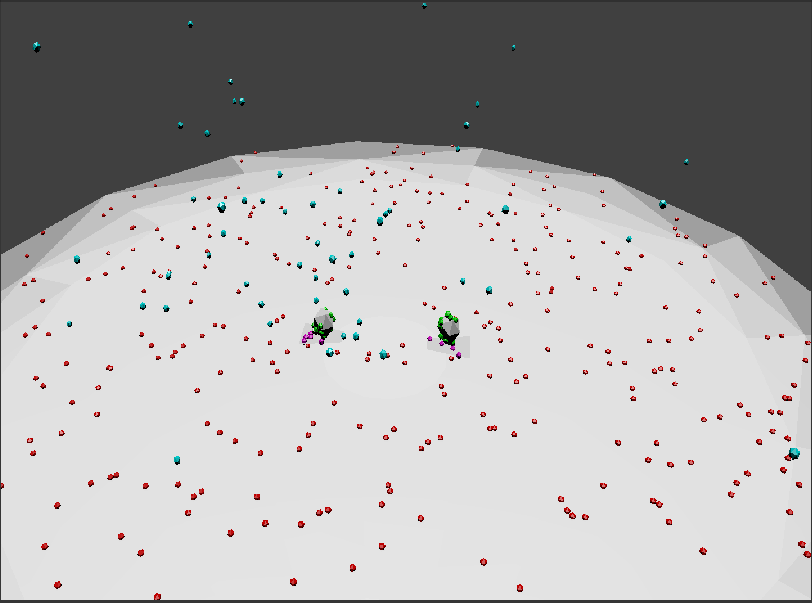
\includegraphics[scale = 0.4]{fig1.png} % requires the graphicx package
   \caption{State of the synapse prior to vesicle release}
   \label{fig1}
\end{figure}

\begin{figure}[H]
   \centering
   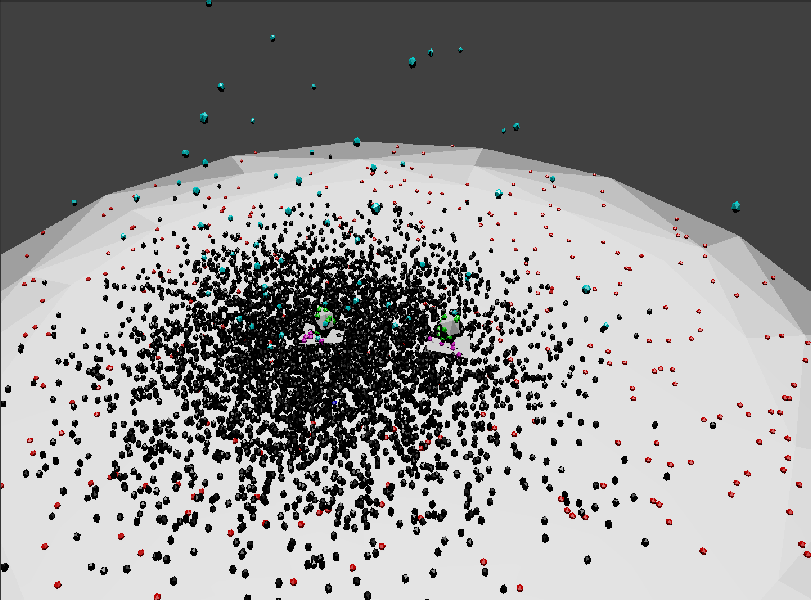
\includegraphics[scale = 0.4]{fig2.png} % requires the graphicx package
   \caption{State of the synapse immediately after vesicle release}
   \label{fig2}
\end{figure}

\section{Conclusion}
We demonstrated in detail a method to model and visualise calcium buffering at nerve terminals. Using CellBlender, MCell, and Python, we were able to create a working model of a spine head and bouton, as well as the vesicle release mechanisms within. This paper was able to extend the methodology provided in \cite{Czech:MethodsMolBiol:2009} by introducing a method (with the help of Mr. Czech himself) to visualise both the presynaptic and postsynaptic parts of the model simultaneously.

Subsequently, we were able to source from the literature the relevant parameters required to set up the model in a realistic fashion. By parameterising the model appropriately, we demonstrate that modelling of this type can produce models which are sufficiently realistic to be useful in answering scientific questions. The model we have set up can be easily extended to answer a different question - this is merely a matter of introducing the appropriate reactions, molecules, and quantities.

\section{Acknowledgements}
The author would like to thank Jacob Czech of the Pittsburgh Supercomputing Centre for his direct assistance in resolving some technical questions regarding the CellBlender addon, as well as Markus Dittrich of the same institution for directing the authors queries to Mr. Czech. The author would also like to thank \cite{Rollehagen::2015} for allowing the use of their morphology data on L5 synaptic connections. Their paper is currently in preparation and is due to be published later this year. Finally, the author would like to thank Christian Stricker for his invaluable help and time in supervising and assisting the author in the writing of this report.

\bibliography{report_doc}{}
\bibliographystyle{cell}



\end{document}
